

\subsection{External Interface Requirements}

\subsubsection{User Interfaces}

Here is shown a mockup of the mobile application UI. The images outline the user interface of the most important screens from the point of view of a generic user, both registered and unregistered. The idea is to implement a easy-to-use mobile application interface, with the possibility to navigate through the pages using a navigation bar and buttons. Further details are provided in the Design Document of the application.

\textbf{User Interfaces for Registered and Unregistered Users}

\begin{figure}[H]

\begin{minipage}{0.45\textwidth}
    \centering
    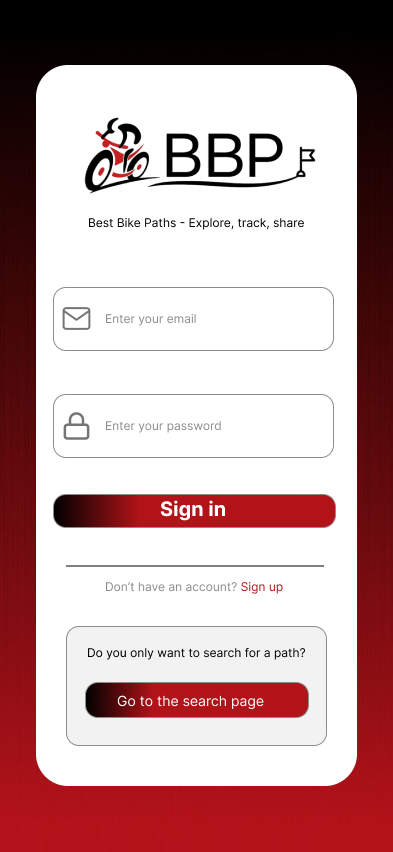
\includegraphics[width=\textwidth]{Images/User Interfaces/Sign in page.png}
    \caption{Sign in page of BBP.}
\end{minipage}
\hspace{1 cm}
\begin{minipage}{0.45\textwidth}
    \centering
    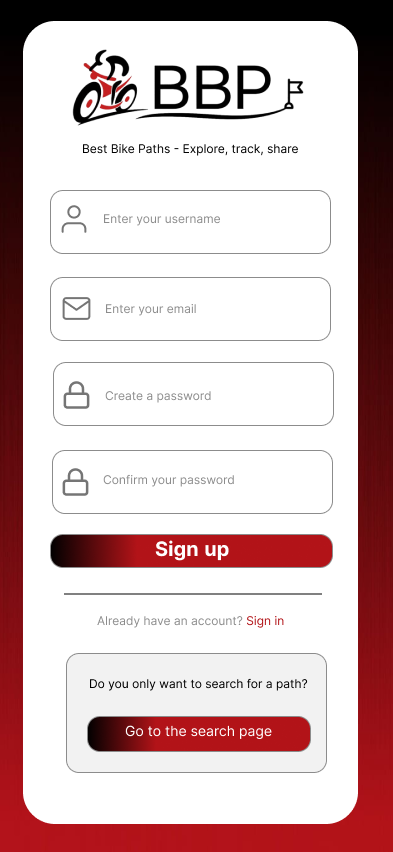
\includegraphics[width=\textwidth]{Images/User Interfaces/Sign up page.png}
     \caption{Sign up page of BBP.}
\end{minipage}

\end{figure}

\newpage

\begin{figure}[H]

\begin{minipage}[t]{0.45\textwidth}
    \vspace{0 pt}
    \framebox{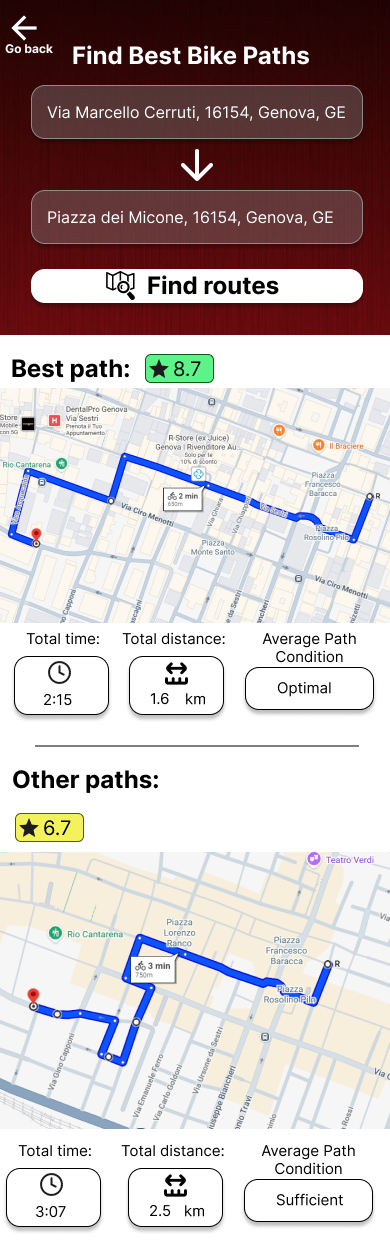
\includegraphics[width=\textwidth]{Images/User Interfaces/Find Best Bike Paths pt.1.png}}
\end{minipage}
\hspace{1 cm}
\begin{minipage}[t]{0.45\textwidth}
    \vspace{0 pt}
   \framebox{ 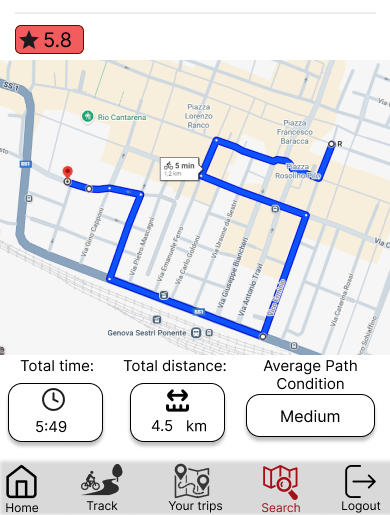
\includegraphics[width=\textwidth]{Images/User Interfaces/Find Best Bike Paths pt.2.png}}
     \caption{Possible screen visualization after a search in BBP. Note: If a User is not registered, the navigation bar is not present}
\end{minipage}

\end{figure}

\newpage

\textbf{User Interfaces for Registered Users only}

\begin{figure}[H]

\begin{minipage}{0.5\textwidth}
    \centering
    \framebox{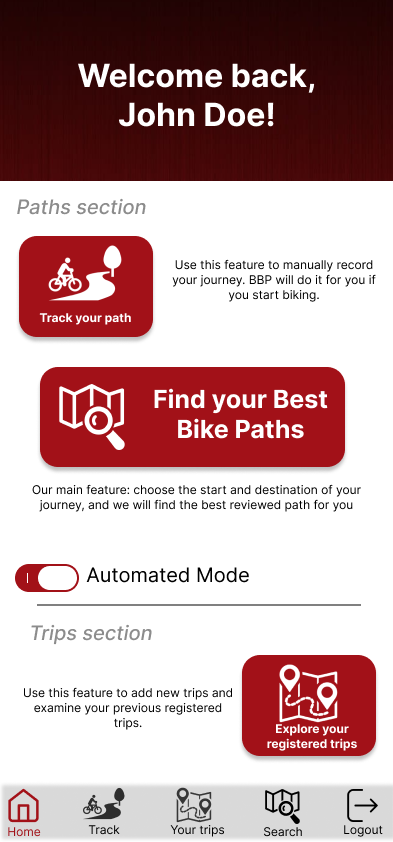
\includegraphics[width=\textwidth]{Images/User Interfaces/Home Page.png}}
    \caption{Home page of BBP.}
\end{minipage}
\hspace{1 cm}
\begin{minipage}{0.5\textwidth}
    \centering
    \framebox{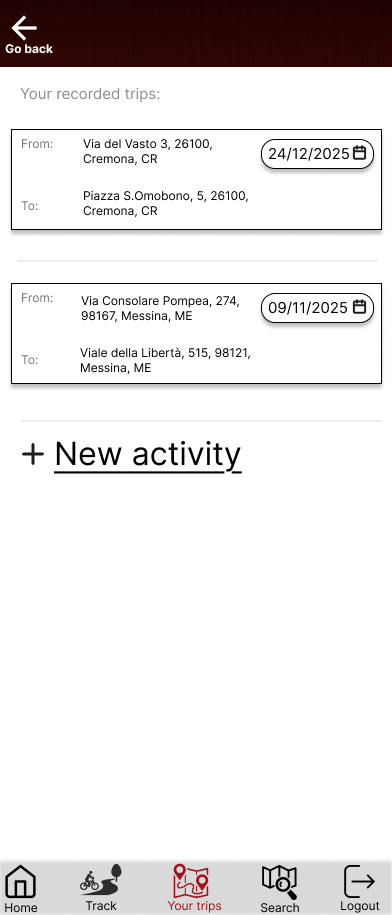
\includegraphics[width=\textwidth]{Images/User Interfaces/Seeing your trips.png}}
     \caption{List of trips registered (not published paths).}
\end{minipage}

\end{figure}

\newpage

\begin{figure}[H]

\begin{minipage}{0.45\textwidth}
    \centering
    \framebox{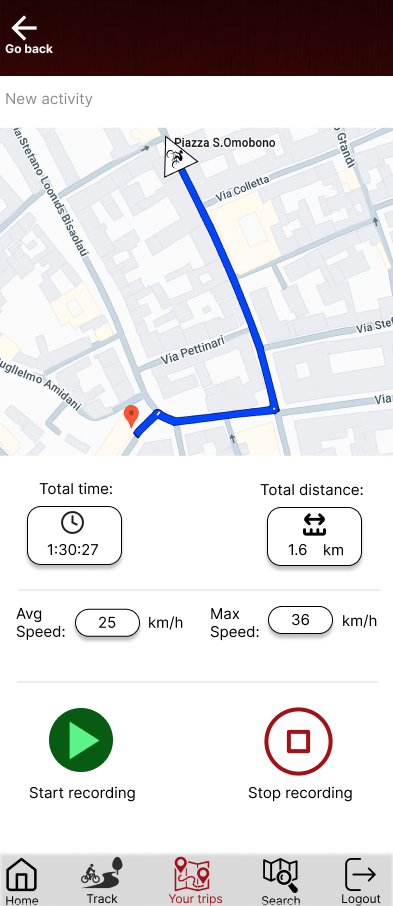
\includegraphics[width=\textwidth]{Images/User Interfaces/Adding new activity.png}}
    \caption{Recording a new activity using BBP.}
\end{minipage}
\hspace{1 cm}
\begin{minipage}{0.45\textwidth}
    \centering
    \framebox{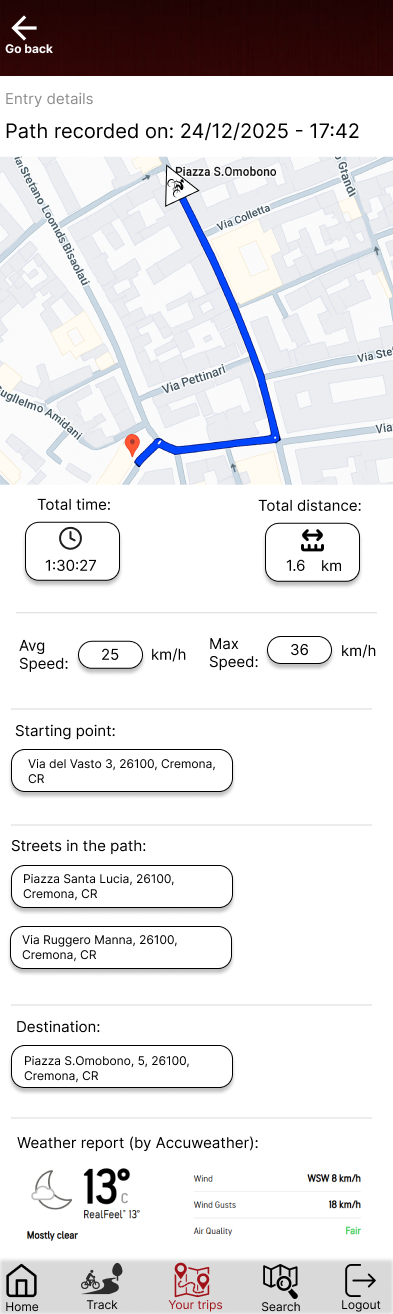
\includegraphics[width=\textwidth]{Images/User Interfaces/Entry details.png}}
     \caption{Reviewing your recorded activities using BBP.}
\end{minipage}
\end{figure}

\newpage

\begin{figure}[H]
\centering
\framebox{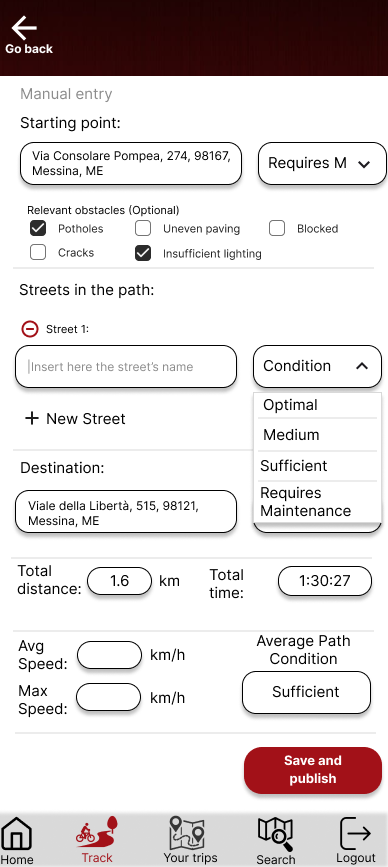
\includegraphics[width=0.5\textwidth]{Images/User Interfaces/Tracking page manual.png}}
\caption{Page used to insert tracked paths to be published and made available to every user.}
\end{figure}

\newpage

\begin{figure}[H]

\begin{minipage}{0.5\textwidth}
    \centering
    \framebox{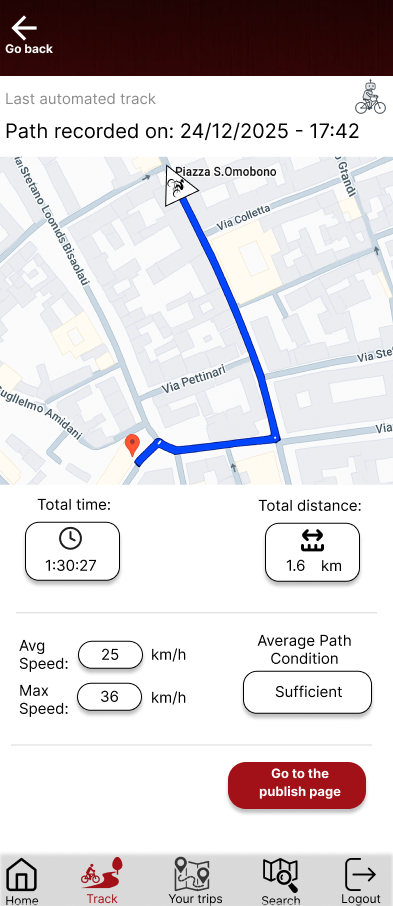
\includegraphics[width=\textwidth]{Images/User Interfaces/Tracking automated.png}}
    \caption{After doing an automated tracking of a path, this is the first screen the user sees when booting up the app.}
\end{minipage}
\hspace{1 cm}
\begin{minipage}{0.5\textwidth}
    \centering
    \framebox{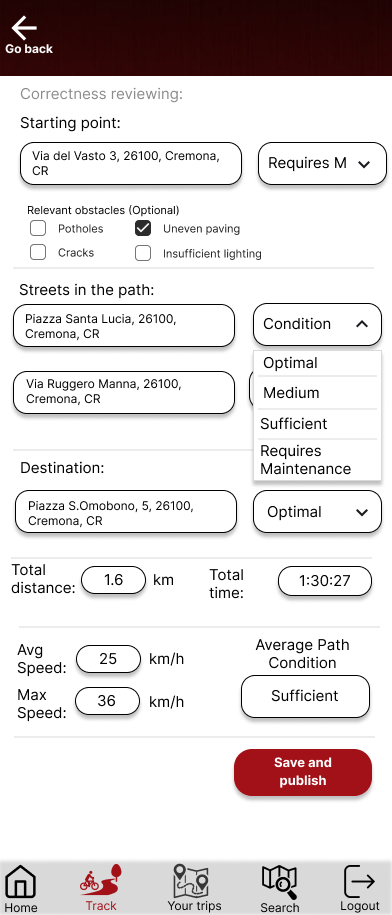
\includegraphics[width=\textwidth]{Images/User Interfaces/Tracking automated publish.png}}
     \caption{Reviewing the automated tracking paths before publishing them.}
\end{minipage}
\end{figure}

\subsubsection{Hardware Interfaces}

Our platform is a mobile application, requiring a portable device, such as a smartphone. Additional sensors are mandatory (either inside the device or connectable to be easily read by it):
\begin{itemize}
    \item \textbf{GPS}: used to gather reliable information regarding the biker's position in the map. It is needed to also accurately reconstruct the path performed by the user.
    \item \textbf{Gyroscope}: used to gather reliable information regarding the possible obstacles in the path (e.g. potholes).
    \item \textbf{Accelerometer}: used to gather reliable information regarding the possible obstacles in the path, the user's speed during the activity (maximum and average speed) and detect when the biker is starting or ending their activity (in automated mode).
\end{itemize}
A stable Internet connection is also required throughout the entirety of the recording, in particular during the saving of the recordings and the queries to search the best possible paths (both of these features require communication with the central server).

\subsubsection{Software Interfaces}
\subsubsection*{Email and Weather Report Systems}
In order to enrich the user experience, an external email delivery system ~\cite{aws_ses_2025} is used to send confirmation emails. Furthermore, trip data can be enriched by weather report systems ~\cite{OpenWeatherMapAPI}. To achieve this, the system relies on REST APIs as interfaces to the explained services and components.

\subsubsection*{Map rendering}
To make the user interface more accessible, a mapping SDK~\cite{MapsSDK} is used by BBP to show on-screen a map of the current location and the possible paths. The SDK provides APIs to draw tiles, overlays, pointers.

\subsubsection*{DBMS}
In order to store the entirety of the information that makes BPP work, a database and a management system is needed. Every DBMS provides APIs to perform actions to the data.

\subsubsection{Communication Interfaces}
Our system consists of two main parts: the mobile application and the backend system, that also communicate with several others components.

\subsubsection*{Communication between mobile application and system}
The mobile application must communicate with the backend system using the Internet protocols. This means that each interaction, in particular data transmission, must be secure and encrypted using REST APIs with HTTPS.
The purpose of this connection is in regard of the entirety of the user authentication process, the upload and the download of trip and path information.

\subsubsection*{Communication between mobile application and on-device sensors}
The mobile application must communicate with on-device sensors to retrieve data to be sent to the server, here stored, processed and made available to others. This communication happens through specific APIs for each and every sensor.

\subsubsection*{Communication between server and email provider}
The server must communicate with an email delivery system to send profile confirmation emails. For this purpose, REST APIs with HTTPS are still widely used. It is to note that the mobile application never communicates with the email provider system, all of the actions go through the server.

\subsubsection*{Communication between server and weather provider}
The server must communicate with an external weather providing system to send queries about current weather reports and receive data to attach to trip information. For this purpose, REST APIs with HTTPS are still widely used. It is to note that the mobile application never communicates with the weather report system, all of the actions go through the server.

\subsubsection*{Communication between server and database}
The server must communicate with a database system, to store and retrieve data about users, paths and trips. For this purpose, SQL queries are the basis of our communication.

\subsection{Functional Requirements}

\begin{enumerate}[label=•  R\arabic*:]

\subsubsection*{Sign up}

    \item The system must allow users to register using a username, an email and a password.
    \item The system must verify that credentials are unique.
    \item The system must send a verification email to the user.
    \item The system must let people verify their email after receiving the verification request.
    \item The system must activate accounts only if verified.

\subsubsection*{Login and Logout}
    \item The system must allow registered users to log in using email and password.
    \item The system must verify the correctness of the credentials.
    \item The system must allow registered users to log in only if the credentials are correct.
    \item The system must allow registered users, that logged-in, to log out.
    \item The system must delete user's session.
    \item The system must allow only registered users to record trips and submit new bike path information.
    \item The system must allow every user to access the system to browse paths.

\subsubsection*{Permissions}
    \item The system must ask registered users to give permissions for the sensors.
    \item The system must read the sensors data only if the permissions are given by the registered user.

\subsubsection*{Trip Management}

    \item The system must allow registered users to record their bike trips.
    \item The system must use sensors to track the biker's trip and their performance metrics.
    \item The system must allow the registered user to save the trip recorded.
    \item The system must check the availability of the Weather Reporting Service (WRS) before requesting data.
    \item The system must ask the WRS for weather information regarding the trip considered.
    \item The system must attach weather information to the trip entry, if available.
    \item The system must show registered users a list of their recorded trips.
    \item The system must allow registered users to see details of a specified recorded trip.

\subsubsection*{Bike Path Management - Manual mode}

    \item The system must allow registered users to manually insert path information using a form.
    \item The system must require the user to specify roads and intersections in the path.
    \item The system must allow registered users to specify the condition of each road in the path.
    \item The system must allow registered users to report additional issues (f.e. potholes).
    \item The system must save the path information in the central database.

\subsubsection*{Bike Path Management - Automated mode}
    \item The system must let registered users enable automated mode.
    \item The system must let registered users disable automated mode.
    \item The system must let registered users add path information via automated mode.
    \item The system must record data using sensors only if automated mode is enabled.
    \item The system must recognize if the registered user is biking.
    \item The system must start recording the path only if the system recognizes that the registered user is biking.
    \item The system must use the sensors' data to record the path.
    \item The system must record intersections and road crossed by the registered user.
    \item The system must recognize obstacles in the path (f.e. pothole) using sensors' data.
    \item The system must recognize if the registered user stopped biking.
    \item The system must stop recording the path if the system recognizes that the registered user stopped biking.
    \item The system must save the recorded bike path information in "to be reviewed" state after an automated mode recording
    \item The system must notify the user that a path has been recorded this way.
    \item The system must require registered users to review and edit information collected via automated mode before publishing.
    \item The system must allow registered users to discard the information collected via automated mode.
    \item The system must allow registered users to save and publish the information recorded via automated mode.
    

\subsubsection*{Finding the Best Path}
    \item The system must allow every user, regardless of their registration status, to browse for paths.
    \item The system must allow the user to fill up a form regarding an origin and destination point.
    \item The system must compute the best path(s) considering the specified points.
    \item The system must merge information from multiple users regarding a road, considering freshness of information and number of confirming users.
    \item The system must compute an average status for the specified path.
    \item The system must compute a score for the specified path, considering their status and the easy reachability.
    \item The system must show the user all the possible best paths in descendant score order, with their scores and metrics.
    \item The system must show the user a map of the best path(s).
\end{enumerate}

\subsubsection{Use Case Diagram ~\cite{UMLUseCaseDiagrams}} 
\begin{figure}[H]
\centering
\framebox{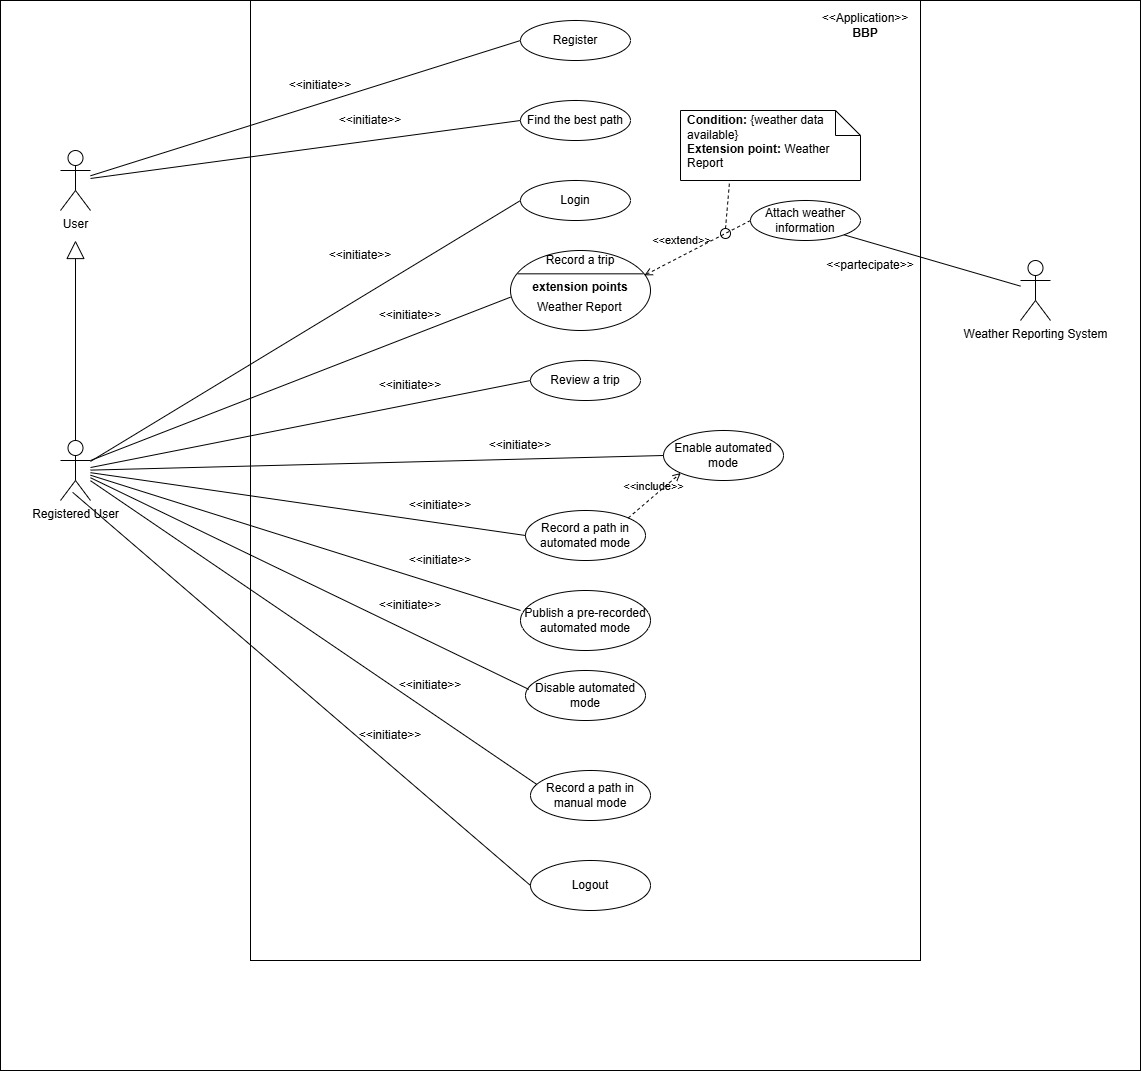
\includegraphics[width=\textwidth]{Images/Diagrams/Use Case/Use Case Diagram.jpg}}
\caption{Use Case Diagram}
\end{figure}
\newpage

\subsubsection{Use Cases}

\begin{enumerate}[label=\textbf{[UC\arabic*]}]

    \item \textbf{Register}
        \begin{center}
            \begin{tabular}{|p{4cm}|p{11cm}|}
                \hline
                \textbf{Name} & \textbf{Register} \\
                \hline
                Actors & User \\
                \hline
                Entry Condition & User opens the BBP platform \\
                \hline
                Event Flow & 
                1. The user presses "Don't have an account? Sign up" in the first page\\
                & 2. The system requires the user to fill out a form with the user's username, email address, and a password.\\
                & 3. The user inserts username, email address, and a password.\\
                & 4. The user presses the "Sign Up" button\\
                & 5. The system verifies that: \newline -the username does not exist yet \textbf{AND},\newline -the email address has not been registered yet. \\
                & 6. The system sends a verification email to the provided address.\\
                & 7. Outside the system, the user verifies the email address (provided in step 3) by clicking the link inside the email sent in step 6. \\
                \hline
                Exit Condition & The user has successfully registered to the platform \\
                \hline
                Exception & E1 - (6) The email cannot be delivered to the provided email address.\newline The system tries to send the email again and displays an error to the user if it fails again \\
                & E2 - (5) The username already exists.\newline In this case, the system displays an error to the user and asks them to try with another username. \\
                & E3 - (5) The email already exists.\newline In this case, the system display an error to the user and asks them to try with another email or if they want to login instead. \\
                \hline
            \end{tabular}
            \captionof{table}{Organization Registration Use Case}
        \end{center}
\newpage
    \item \textbf{Find the best path}
        \begin{center}
            \begin{tabular}{|p{4cm}|p{11cm}|}
                \hline
                \textbf{Name} & \textbf{Find the Best Path} \\
                \hline
                Actors & User \\
                \hline
                Entry Condition & One of the following conditions must hold: \newline -User opens the BBP platform \textbf{OR} \newline -User is in the home page\\
                \hline
                Event Flow & 1. The user initiates the route search by pressing one of the following buttons:\newline -"Go to the search page" \textbf{OR} \newline -"Find your Best Bike Paths" \textbf{OR} \newline -"Search" in the navigation bar. \\
                & 2. The system requires the user to insert an origin and a destination point. \\
                & 3. The user inserts the origin and destination point. \\
                & 4. The user presses the "Find routes" button.\\
                & 5. The system merges information from different users, considering freshness and number of confirming users.\\
                & 6. The system computes possible bike paths and their score between these points. \\
                & 7. The system displays paths and their scores in descendant score order. \\
                \hline
                Exit Condition & The user sees recommended bike paths with visualized scores and information about riding time, total distance and path condition. \\
                \hline
                Exception & E1 - (6) No valid path between selected points. \newline In this case, the system will provide the user with a blank page and a message saying that there not exists a path between those two points. \\
                & E2 - (6) System fails to retrieve path data.\newline In this case, the system tries again and, if not possible, warns the user to try again later. \\
                \hline
            \end{tabular}
            \captionof{table}{Find the best path Use Case}
        \end{center}
    
    \item \textbf{Login} 
        \begin{center}
            \begin{tabular}{|p{4cm}|p{11cm}|}
                \hline
                \textbf{Name} & \textbf{Login} \\
                \hline
                Actors & Registered User \\
                \hline
                Entry Condition & Registered user opens the platform \\
                \hline
                Event Flow & 1. The system prompts the registered user to enter email and password credentials. \\
                & 2. The registered user enters email and password credentials. \\
                & 3. The registered user presses the "Sign in" button. \\
                & 4. The system verifies validates entered credentials \\
                \hline
                Exit Condition & The registered user has successfully logged in to the platform \\
                \hline
                Exception & E1: (4) - Invalid credentials. \newline In this case, the system displays an error message "Invalid email or password" and prompts the registered user to try again.\\
                & E2: (4) - Email address not verified. \newline In this case, the system informs the registered user that the email has not been verified and prompts to try again.\\
                \hline
            \end{tabular}
            \captionof{table}{Login Use Case}
        \end{center}
\newpage
    \item \textbf{Record a Trip} 
        \begin{center}
            \begin{tabular}{|p{4cm}|p{11cm}|}
                \hline
                \textbf{Name} & \textbf{Record a trip} \\
                \hline
                Actors & Registered User \\
                \hline
                Entry Condition & Registered user is logged in \\
                \hline
                Event Flow & 1. The registered user goes to the registered trips section by: \newline -pressing the "Track your path" button \textbf{OR},\newline -pressing the "Your Trips" button in the navigation bar.\\
                & 2. The registered user presses the "New Activity" button. \\
                & 3. The system displays the “New Activity” page, prompting the user to start recording.\\
                & 4. The registered user presses the "Start recording" button. \\
                & 5. The system starts recording the trip, collecting GPS location, speed, and sensor data. \\
                & 6. The registered user can pause or resume the recording. \\
                & 7. The registered user stops the recording. \\
                & 8. The system saves the trip information and displays a summary including total time, average speed, and total distance. \\
                \hline
                Exit Condition & Trip is stored with performance metrics \\
                \hline
                Exception & E1: (5) - GPS/sensor data not available\newline In this case, the system displays an error to the registered user, describing the problem and suggesting to check the sensors or try again another time. \\
                & E2: (8) Error saving the data into the system\newline In this case, the system tries to save again until it is successfully saved. \\
                & E3: (5) The application crashes during the recording\newline In this case, the system pauses the recording and, at the reboot of the application, prompts the registered user to save it or start it again. \\
                & E4: (4) Permissions not granted\newline The system prompts the registered user for access to the sensors and background execution. If the registered user denies permissions, the system disables automated mode and notifies the registered user.\\
                \hline
                Extension Point: & Step 8 - Optional: Trigger Weather Report\\
                \hline
            \end{tabular}
            \captionof{table}{Record a trip Use Case}
        \end{center} 

    \item \textbf{Attach weather information} 
        \begin{center}
            \begin{tabular}{|p{4cm}|p{11cm}|}
                \hline
                \textbf{Name} & \textbf{Attach weather information} \\
                \hline
                Actors & Weather Reporting System (WRS) \\
                \hline
                Entry Condition & A trip without weather data is recorded \\
                \hline
                Event Flow & 1. The system checks the availability of the Weather Reporting System (WRS). \\
                & 2. The WRS responds with its availability. \\
                & 3. The system requests contextual weather data for the trip from the WRS. \\
                & 4. The WRS provides meteorological information, including wind speed, temperature, and weather conditions. \\
                & 5. The system attaches the received weather information to the trip record. \\
                \hline
                Exit Condition & Trip is stored with performance metrics and weather information \\
                \hline
                Exception & E1 - (1) WRS not available.\newline In this case, the system acts like no weather information were available and does not attach anything to the trip. \\
                & E2 - (3) Weather data not available.\newline In this case, the system does not attach anything to the trip information.\\
                \hline
            \end{tabular}
            \captionof{table}{Attach weather information Use Case}
        \end{center}
\newpage
    \item \textbf{Review a trip} 
        \begin{center}
            \begin{tabular}{|p{4cm}|p{11cm}|}
                \hline
                \textbf{Name} & \textbf{Review a Trip} \\
                \hline
                Actors & Registered User \\
                \hline
                Entry Condition & Registered user is logged in \\
                \hline
                Event Flow & 1. The registered user goes to the registered trips section by: \newline -pressing the "Explore your registered trips" button \textbf{OR},\newline -pressing the "Your Trips" button in the navigation bar.\\
                & 2. The system displays a list of recorded trips, showing the starting and finishing points, and the date of each trip. \\
                & 3. The registered user presses on a trip. \\
                & 4. The system displays a detailed view with the information of the selected trip, including all recorded information.. \\
                \hline
                Exit Condition & The registered user reviews trip data. \\
                \hline
                Exception & E1 - No registered trip associated with the registered user. \newline In this case, the system shows an empty page to the registered user.\\
                 & E2 - Error fetching trip information \newline In this case, the system displays an error message to the registered user, inviting to try again later.\\
                \hline
            \end{tabular}
            \captionof{table}{Review a trip Use Case} 
        \end{center} 


    \item \textbf{Record a Path in Automated Mode}
            \begin{center}
                \begin{tabular}{|p{4cm}|p{11cm}|}
                    \hline
                    \textbf{Name} & \textbf{Record a Path in Automated Mode} \\
                    \hline
                    Actors & Registered User \\
                    \hline
                    Entry Condition & All of these conditions must hold: \newline -Registered user is logged in \textbf{AND}, \newline -Automated mode is enabled.\\
                    \hline
                    Event Flow & 1. The registered user begins a bike ride with automated mode already enabled -> see ~\hyperref[EAM]{Enable Automated Mode} \\
                    & 2. The system records GPS, accelerometer, and gyroscope data while the user is cycling. \\
                    & 3. The system detects possible obstacles or potholes from sensor data and saves the information. \\
                    & 4. The registered user stops biking. \\
                    & 5. The system detects when the user ended the bike ride. \\
                    & 6. The system saves the recorded bike path information \\
                    & 7. The system notifies the registered user that a new path has been recorded. \\
                    \hline
                    Exit Condition & Path information is stored and is ready for review. \\
                    \hline
                    Exception & E1: (2) - GPS/sensor data not available\newline In this case, the system displays an error to the registered user, describing the problem and suggesting to check the sensors or try again another time. \\
                    & E2: (6) Error saving the data into the system\newline In this case, the system tries to save again until it is successfully saved. \\
                    & E3: (2) The application crashes during the recording\newline In this case, the system stops the recording and, at the reboot of the application, acts as if the recording has ended normally. \\
                    \hline
                \end{tabular}
                \captionof{table}{Record a Path in Automated Mode Use Case}
            \end{center}
\newpage
    \item \textbf{Enable Automated Mode}
        \label{EAM}
        \begin{center}
            \begin{tabular}{|p{4cm}|p{11cm}|}
                \hline
                \textbf{Name} & \textbf{Enable Automated Mode} \\
                \hline
                Actors & Registered User \\
                \hline
                Entry Condition & Registered user is logged in \\
                \hline
                Event Flow & 1. The registered user presses the toggle button "Automated mode" \\
                & 2. The system starts collecting data from the device's sensors (GPS, accelerometer, gyroscope) \\
                & 3. The system notifies the registered user that automatic mode is enabled. \\
                \hline
                Exit Condition & The system actively collects bike path and sensor data \\
                \hline
                Exception & E1: (1) Permissions not granted\newline The system prompts the user for access to the sensors and background execution. If the user denies permissions, the system disables automated mode and notifies the user. \\
                &  E2: (2) - GPS/sensor error\newline In this case, the system displays an error to the user, describing the problem and suggesting to check the sensors or try again another time. \\
                \hline
            \end{tabular}
            \captionof{table}{Enable Automated Mode Use Case}
        \end{center}

    \item \textbf{Disable Automated Mode}
        \begin{center}
            \begin{tabular}{|p{4cm}|p{11cm}|}
                \hline
                \textbf{Name} & \textbf{Disable Automated Mode} \\
                \hline
                Actors & Registered User \\
                \hline
                Entry Condition & All of these conditions must hold: \newline -Registered user is logged in \textbf{AND}, \newline -Automated mode is enabled.\\
                \hline
                Event Flow & 1. The registered user presses the toggle button "Automated mode" \\
                & 2. The system stops collecting data from the device's sensors (GPS, accelerometer, gyroscope) \\
                & 3. The system notifies the registered user that automatic mode is disabled. \\
                \hline
                Exit Condition & System is no longer collecting bike path and sensor data \\
                \hline
                Exception & E1: (1) Trip/Path recording in progress \newline 
                In this case, the system stops recording the trip/path. \\
                &  E2: (2) - GPS/sensor error\newline In this case, the system displays an error to the registered user, describing the problem and suggesting to check the sensors or try again another time. \\
                \hline
            \end{tabular}
            \captionof{table}{Disable Automated Mode Use Case}
        \end{center}
\newpage
        \item \textbf{Publish a pre-recorded automated mode path}
        \begin{center}
            \begin{tabular}{|p{4cm}|p{11cm}|}
                \hline
                \textbf{Name} & \textbf{Publish a pre-recorded automated mode path} \\
                \hline
                Actors & Registered User \\
                \hline
                Entry Condition & Registered user is logged in, automated mode is enabled, and a path has been recorded \\
                \hline
                Event Flow & 1. The system notifies the registered user that a new path has been recorded and is ready to be reviewed. \\
                & 2. The user accesses the recorded path by either pressing the notification \textbf{OR} opening the application after ending the recording. \\
                & 3. The system displays the recorded path information \\
                & 4. The system prompts the registered user to either confirm, edit, or delete the recorded path information.\\
                & 5. The registered user reviews and, if necessary, edits the path information. \\
                & 6. The registered user presses "Save and publish". \\
                & 7. The system saves the path information in the central database, making it available for other users. \\
                \hline
                Exit Condition & Path information is stored and is published \\
                \hline
                Exception & E1: (4) The registered user deletes the recording.\newline In this case, the recording is discarded.\\
                & E2: (7) Error saving the data into the system\newline In this case, the system tries to save again until it is successfully saved. \\
                \hline
            \end{tabular}
            \captionof{table}{Publish a pre-recorded automated mode path Use Case}
        \end{center}

    \item \textbf{Record a Path in Manual Mode}
        \begin{center}
            \begin{tabular}{|p{4cm}|p{11cm}|}
                \hline
                \textbf{Name} & \textbf{Record a Path in Manual Mode} \\
                \hline
                Actors & Registered User \\
                \hline
                Entry Condition & Registered user is logged in \\
                \hline
                Event Flow & 1. The registered user goes to the registered trips section by: \newline -pressing the "Track your path" button \textbf{OR},\newline -pressing the "Track" button in the navigation bar.\\
                & 2. The system prompts the registered user to provide path information via a form. \\
                & 3. The registered user fills out the form with the streets and intersections forming the path, specifying the status of each road and detailing any issues if the road is not optimal.\\
                & 4. The registered user presses "Save and publish" \\
                & 5. The system saves the path information in the central database, making it publicly available for other users. \\
                \hline
                Exit Condition & Path information is stored and can be made publishable \\
                \hline
                Exception & E1: (3) Mandatory data not provided \newline In this case, the system displays a message to the registered user, prompting them to add the missing details. \\
                & E2: (7) Error saving the data into the system\newline In this case, the system tries to save again until it is not saved. \\
                & E3: (4) The registered user deletes the entry\newline In this case, the system discards the path. \\
                \hline
            \end{tabular}
            \captionof{table}{Record a path in manual mode Use Case}
        \end{center}
\newpage
        \item \textbf{Logout}
        \begin{center}
            \begin{tabular}{|p{4cm}|p{11cm}|}
                \hline
                \textbf{Name} & \textbf{Logout} \\
                \hline
                Actors & Registered User \\
                \hline
                Entry Condition & Registered user is logged in. \\
                \hline
                Event Flow & 1. Registered user presses "Logout" on the navigation bar. \\
                & 2. The system prompts the registered user to confirm the logout action. \\
                & 3. The registered user confirms. \\
                & 4. The system revokes the user’s session credentials and clears all session-related data.\\
                & 5. The system redirects the user to the login page. \\
                \hline
                Exit Condition & Registered user is no longer authenticated; session is closed \\
                \hline
                Exception & E1: (4) Error to terminate session correctly. \newline In this case, the system retries to terminate session correctly until it is possible.\\
                & E2: (2) The registered user cancels the logout action.\newline In this case, the system redirects the registered user to the home page.\\
                \hline
            \end{tabular}
            \captionof{table}{Logout Use Case}
        \end{center}
    
\end{enumerate}
\subsubsection{Mapping}

\begin{table}[H]
\begin{tabular}{|p{5cm}|p{5cm}|p{5cm}|}
\hline
\textbf{Goal} & \textbf{Requirements and Domain\newline Assumptions} & \textbf{Use cases}\\
\hline
\textbf{G1}: Users can register and have a profile in BBP application. & \begin{tabular}[c]{@{}p{5cm}@{}} \textbf{R1}: The system must allow users to register using a username, an email and a password.\\ \hline \textbf{R2}: The system must verify that credentials are unique. \\ \hline \textbf{R3}: The system must send a verification email to the user. \\ \hline \textbf{R4}: The system must let people verify their email after receiving the verification request. \\ \hline \textbf{R5}: The system must activate accounts only if verified. \\ \hline \textbf{R6}: The system must allow registered users to log in using email and password.\\ \hline \textbf{R7}: The system must verify the correctness of the credentials.\\ \hline \textbf{R8}: The system must allow registered users to log in only if the credentials are correct. \\ \hline \textbf{R9}: The system must allow registered users, that logged-in, to log out. \\ \hline \textbf{R10}: The system must delete user’s session.\\ \hline \hline \textbf{D2}: The internet connection remains relatively stable throughout the session. \\ \hline \textbf{D13}: Users will give non-misleading information about their identity. \end{tabular} & \begin{tabular}[c]{@{}p{5cm}@{}}\textbf{UC1}: Register\\ \hline \textbf{UC3}: Login \\ \hline \textbf{UC12}: Logout\end{tabular}\\
\hline
\end{tabular}
\end{table}


\begin{table}[H]
\begin{tabular}{|p{5cm}|p{5cm}|p{5cm}|}
\hline
\textbf{Goal} & \textbf{Requirements and Domain\newline Assumptions} & \textbf{Use cases}\\
\hline
\textbf{G2}: Users manually create bike paths in an inventory by specifying the name of the streets and the status. & \begin{tabular}[c]{@{}p{5cm}@{}} \textbf{R23}: The system must allow registered users to manually insert path information using a form.\\ \hline \textbf{R24}: The system must require the user to specify roads and intersections in the path. \\ \hline \textbf{R25}: The system must allow registered users to specify the condition of each road in the path. \\ \hline \textbf{R26}: The system must allow registered users to report additional issues (f.e. potholes). \\ \hline \textbf{R27}: The system must save the path information in the central database. \\  \hline \hline \textbf{D2}: The internet connection remains relatively stable throughout the session. \\ \hline \textbf{D4}: Users are expected to provide accurate and non-misleading information when creating new paths. \\ \hline \textbf{D5}: Users do not use the application or the platform for purposes unrelated to biking activities or the exploration of new routes as a recreational activity. \\ \hline \textbf{D8}: The date related to the new inserted path is correct. \\ \hline \textbf{D9}: The app is used where bike track already exists. \\ \hline \textbf{D10}: The biking paths have little to no cars presence. \\ \hline \textbf{D11}: The biking paths have speed limits compatible with the average speed of a bike.  \end{tabular} & \begin{tabular}[c]{@{}p{5cm}@{}}\textbf{UC11}: Record a path in manual mode\end{tabular}\\
\hline
\end{tabular}
\end{table}

%-----GOAL 3 TABLES (divided in two because of space-----%
\begin{table}[H]
\begin{tabular}{|p{5cm}|p{5cm}|p{5cm}|}
\hline
\textbf{Goal} & \textbf{Requirements and Domain\newline Assumptions} & \textbf{Use cases}\\
\hline
\textbf{G3}:Users create bike paths in an automated mode where the system acquire data from the user’s mobile device and reconstruct the path. & \begin{tabular}[c]{@{}p{5cm}@{}} \textbf{R13}: The system must ask registered users to give permissions for the sensors.\\ \hline \textbf{R14}: The system must read the sensors data only if the permissions are given by the registered user. \\ \hline \textbf{R28}: The system must let registered users enable automated mode.\\ \hline \textbf{R29}: The system must let registered users disable automated mode. \\ \hline \textbf{R30}: The system must let registered users add path information via automated mode.\\ \hline \textbf{R31}: The system must record data using sensors only if automated mode is enabled. \\ \hline \textbf{R32}:The system must recognize if the registered user is biking.\\ \hline \textbf{R33}: The system must start recording the path only if the system recognizes that the registered user is biking. \\ \hline \textbf{R34}: The system must use the sensors’ data to record the path.\\ \hline \textbf{R35}: The system must record intersections and road crossed by the registered user. \\ \hline \textbf{R36}:The system must recognize obstacles in the path (f.e. pothole) using sensors’ data.\\ \hline \textbf{R37}: The system must recognize if the registered user stopped biking. \\ \hline \textbf{R38}:The system must stop recording the path if the system recognizes that the registered user stopped biking.\\ \hline \textbf{R39}: The system must save the recorded bike path information in "to be reviewed" state after an automated mode recording \\ \hline \textbf{R40}: The system must notify the user that a path has been recorded this way.\\ \hline \textbf{R41}: The system must require registered users to review and edit information collected via automated mode before publishing. \\ \hline \textbf{R42}: The system must allow registered users to discard the information collected via automated mode.\\ \hline \textbf{R43}: he system must allow registered users to save and publish the information recorded via automated mode.\end{tabular} & \begin{tabular}[c]{@{}p{5cm}@{}}\textbf{UC6}: Enable automated mode \\ \hline \textbf{UC7}: Record a path in automated mode. \\ \hline \textbf{UC8}: Publish a pre-recorded automated mode path. \\ \hline \textbf{UC9}: Disable automated mode.  \end{tabular}\\

\end{tabular}
\end{table}

\begin{table}[H]
\begin{tabular}{|p{5cm}|p{5cm}|p{5cm}|}
 & \begin{tabular}[c]{@{}p{5cm}@{}} \textbf{R27}: The system must save the path information in the central database.\\ \hline \hline  \textbf{D1}: Each user rides a bicycle while the application runs in background in case of automated mode. \\ \hline \textbf{D2}: The internet connection remains relatively stable throughout the session. \\ \hline \textbf{D3}: Users are willing to review and refine the automatically collected information gathered by the device in
the automated-mode. \\ \hline \textbf{D4}: Users are expected to provide accurate and non-misleading information when creating new paths. \\ \hline \textbf{D5}: Users do not use the application or the platform for purposes unrelated to biking activities or the exploration of new routes as a recreational activity. \\ \hline \textbf{D6}: Third-parties services provide reliable information to the application.\\ \hline \textbf{D7}: Hardware devices must provide reliable sensor data to the system to let it acquire the right performance data. \\ \hline \textbf{D8}: The date related to the new inserted path is correct. \\ \hline \textbf{D9}: The app is used where bike track already exists. \\ \hline \textbf{D10}: The biking paths have little to no cars presence. \\ \hline \textbf{D11}: The biking paths have speed limits compatible with the average speed of a bike. \\ \hline \textbf{D12}: Users will stop cycling when they want to end the recording of the path. \end{tabular} & \\
\hline
\end{tabular}
\end{table}
\newpage


\begin{table}[H]
\begin{tabular}{|p{5cm}|p{5cm}|p{5cm}|}
\hline
\textbf{Goal} & \textbf{Requirements and Domain\newline Assumptions} & \textbf{Use cases}\\
\hline
\textbf{G4}: Users browse bike paths within the inventory. They can specify an origin and destination and ask the system to visualize the bike path on a map. & \begin{tabular}[c]{@{}p{5cm}@{}} \textbf{R44}: The system must allow every user, regardless of their registration status, to browse for paths.\\ \hline \textbf{R45}: The system must allow the user to fill up a form regarding an origin and destination point. \\ \hline \textbf{R46}: The system must compute the best path(s) considering the specified points. \\ \hline \textbf{R50}: The system must show the user all the possible best paths in descendant score order, with their scores and metrics. \\ \hline \textbf{R51}: The system must show the user a map of the best path(s). \\  \hline \hline \textbf{D2}: The internet connection remains relatively stable throughout the session. \end{tabular} & \begin{tabular}[c]{@{}p{5cm}@{}}\textbf{UC2}: Find the best path.\end{tabular}\\  
\hline
\end{tabular}
\end{table}

\begin{table}[H]
\begin{tabular}{|p{5cm}|p{5cm}|p{5cm}|}
\hline
\textbf{Goal} & \textbf{Requirements and Domain\newline Assumptions} & \textbf{Use cases}\\
\hline
\textbf{G5}: Users record their trips and store them to keep track of their cycling activities.    & \begin{tabular}[c]{@{}p{5cm}@{}} \textbf{R13}: The system must ask registered users to give permissions for the sensors.\\ \hline \textbf{R14}: The system must read the sensors data only if the permissions are given by the registered user. \\ \hline \textbf{R15}: The system must allow registered users to record their bike trips. \\ \hline \textbf{R16}: The system must use sensors to track the biker’s trip and their performance metrics. \\ \hline \textbf{R17}: The system must allow the registered user to save the trip recorded. \\  \hline \hline \textbf{D2}: The internet connection remains relatively stable throughout the session. \\ \hline \textbf{D5}: Users do not use the application or the platform for purposes unrelated to biking activities or the exploration of new routes as a recreational activity. \\ \hline \textbf{D7}:  Hardware devices must provide reliable sensor data to the system to let it acquire the right performance
data. \\ \hline \textbf{D8}: The date related to the new inserted path is correct. \\ \hline \textbf{D9}: The app is used where bike track already exists. \\ \hline \textbf{D10}: The biking paths have little to no cars presence. \\ \hline \textbf{D11}: The biking paths have speed limits compatible with the average speed of a bike.  \end{tabular} & \begin{tabular}[c]{@{}p{5cm}@{}}\textbf{UC4}: Record a trip. \end{tabular}\\
\hline
\end{tabular}
\end{table}

\begin{table}[H]
\begin{tabular}{|p{5cm}|p{5cm}|p{5cm}|}
\hline
\textbf{Goal} & \textbf{Requirements and Domain\newline Assumptions} & \textbf{Use cases}\\
\hline
\textbf{G6}: Users can see for a recorded trip various statistical data of the user performances as well as meteorological information during the respective trip.  & \begin{tabular}[c]{@{}p{5cm}@{}} \textbf{R18}: The system must check the availability of the Weather Reporting Service (WRS) before requesting data.\\ \hline \textbf{R19}: The system must ask the WRS for weather information regarding the trip considered. \\ \hline \textbf{R20}: The system must attach weather information to the trip entry, if available. \\ \hline \textbf{R21}: The system must show registered users a list of their recorded trips. \\ \hline \textbf{R22}: The system must allow registered users to see details of a specified recorded trip. \\  \hline \hline  \textbf{D6}: Third-parties services provide reliable information to the application. \\ \hline \textbf{D8}: The date related to the new inserted path is correct.  \end{tabular} & \begin{tabular}[c]{@{}p{5cm}@{}}\textbf{UC5}: Attach weather information. \\ \hline \textbf{UC6}: Review a trip.\\ \hline \end{tabular}\\
\hline
\end{tabular}
\end{table}

\begin{table}[H]
\begin{tabular}{|p{5cm}|p{5cm}|p{5cm}|}
\hline
\textbf{Goal} & \textbf{Requirements and Domain\newline Assumptions} & \textbf{Use cases}\\
\hline
\textbf{G7}: The system uses information published by the users about the paths by merging pieces of information to
generate the optimal path, using the freshness and number of confirmed data.  & \begin{tabular}[c]{@{}p{5cm}@{}} \textbf{R47}: The system must merge information from multiple users regarding a road, considering freshness of information and number of confirming users.\\ \hline \textbf{R48}: The system must compute an average status for the specified path. \\ \hline \textbf{R49}: The system must compute a score for the specified path, considering their status and the easy reachability. \\  \hline \hline \textbf{D2}: The internet connection remains relatively stable throughout the session.\\ \hline \textbf{D4}: Users are expected to provide accurate and non-misleading information when creating new paths.\\ \hline \textbf{D8}: The date related to the new inserted path is correct. \end{tabular} & \begin{tabular}[c]{@{}p{5cm}@{}}\textbf{UC2}: Find the best path.\end{tabular}\\  
\hline
\end{tabular}
\end{table}

\subsubsection{Sequence Diagrams ~\cite{UMLSequenceDiagrams}}

This subsection presents notifications modeled at a high level to illustrate user interactions. It deliberately omits detailed design, architectural considerations, and synchronization aspects to focus on the conceptual interaction flow rather than implementation specifics.

\begin{enumerate}[label=\textbf{[UC\arabic*]}]

\pagebreak
\item \textbf{Register}
\begin{figure}[H]
\centering
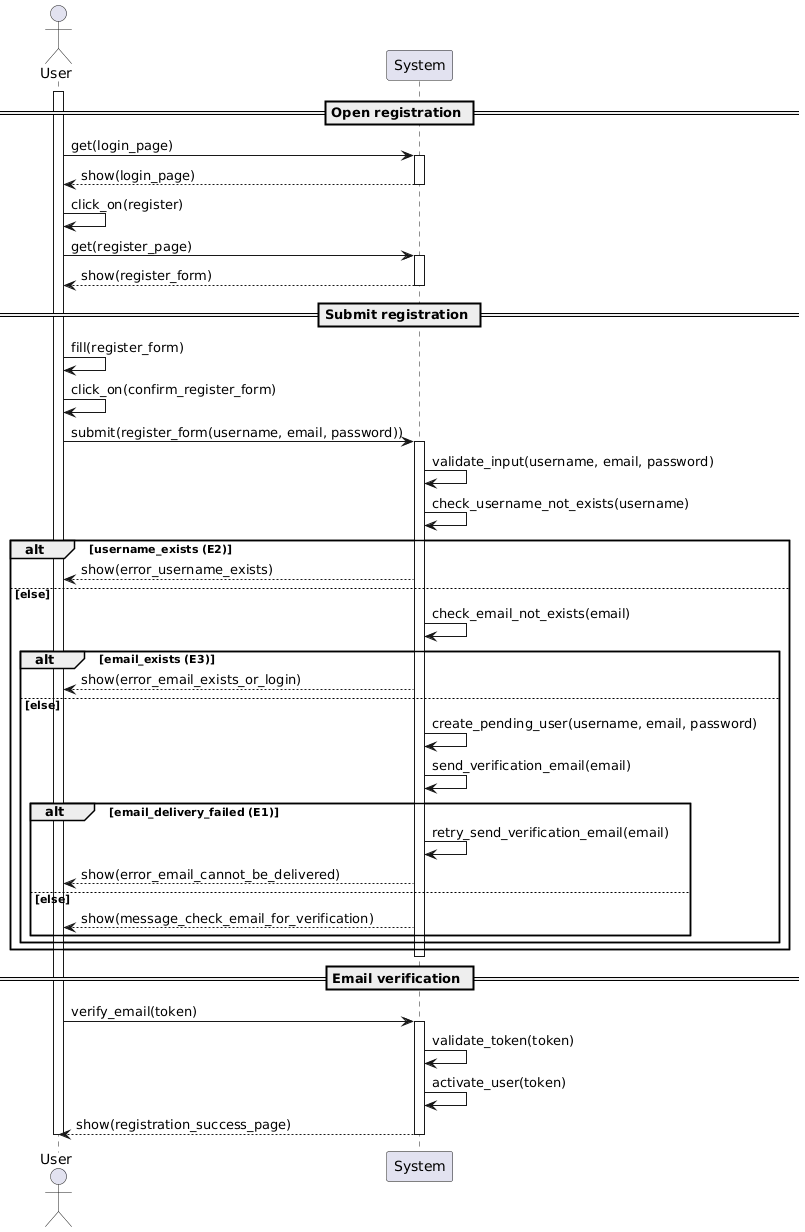
\includegraphics[scale=0.51]{RASD/Images/Diagrams/Sequence/register_sequence.png}
\caption{\label{fig:squencediagram}Sequence diagram for register.}
\end{figure}

\item \textbf{Find the best path}

\begin{figure}[H]
\centering
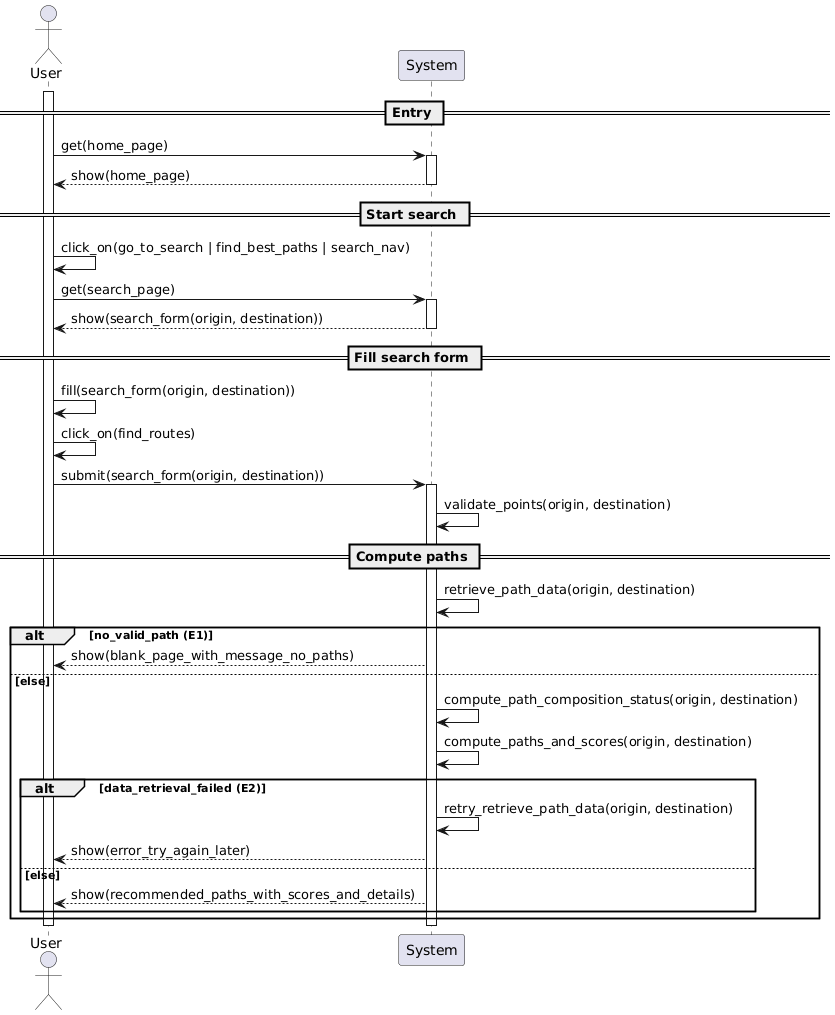
\includegraphics[width=\textwidth]{Images/Diagrams/Sequence/find_best_paths.png}
\caption{\label{fig:squencediagram}Sequence diagram for find best path.}
\end{figure}

\pagebreak

\item \textbf{Login}

\begin{figure}[H]
\centering
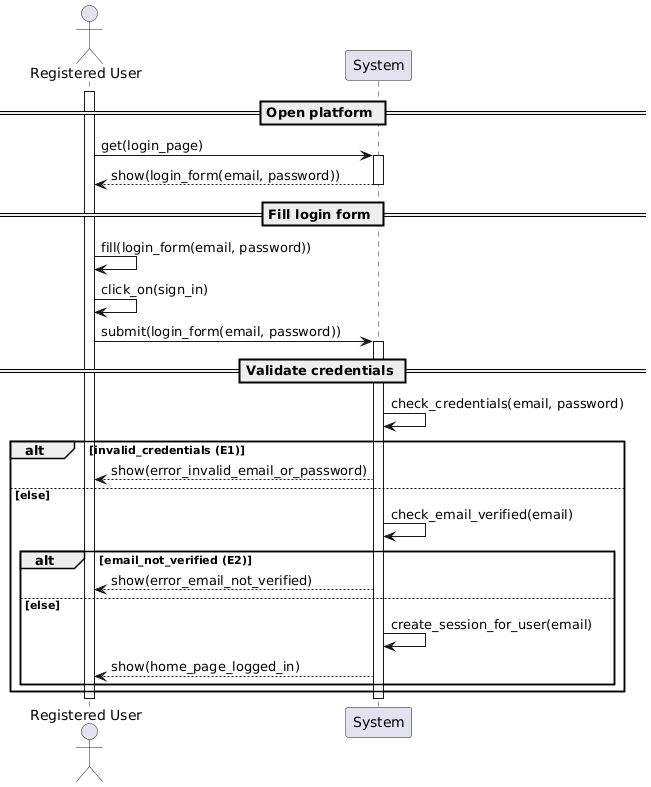
\includegraphics[width=\textwidth]{Images/Diagrams/Sequence/login.png}
\caption{\label{fig:squencediagram}Sequence diagram for login.}
\end{figure}

\pagebreak

\item \textbf{Record a Trip}

\begin{figure}[H]
\centering
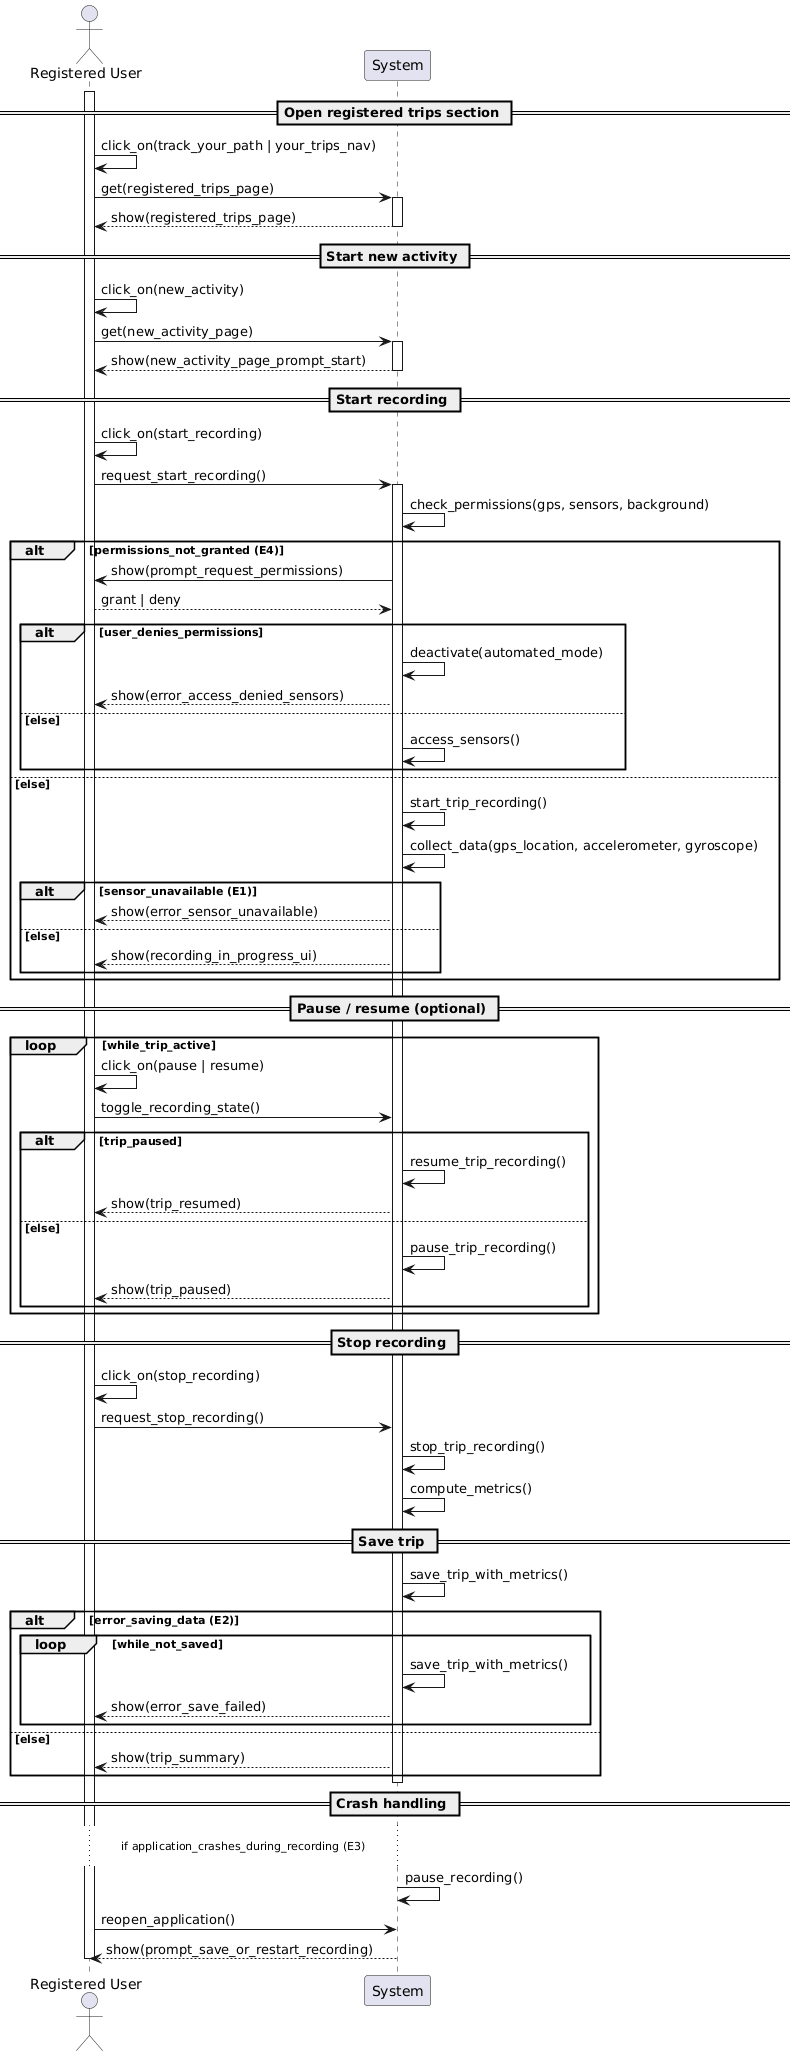
\includegraphics[scale=0.3]{Images/Diagrams/Sequence/record_trip.png}
\caption{\label{fig:squencediagram}Sequence diagram for record trip.}
\end{figure}

\pagebreak

\item \textbf{Attach weather information}

\begin{figure}[H]
\centering
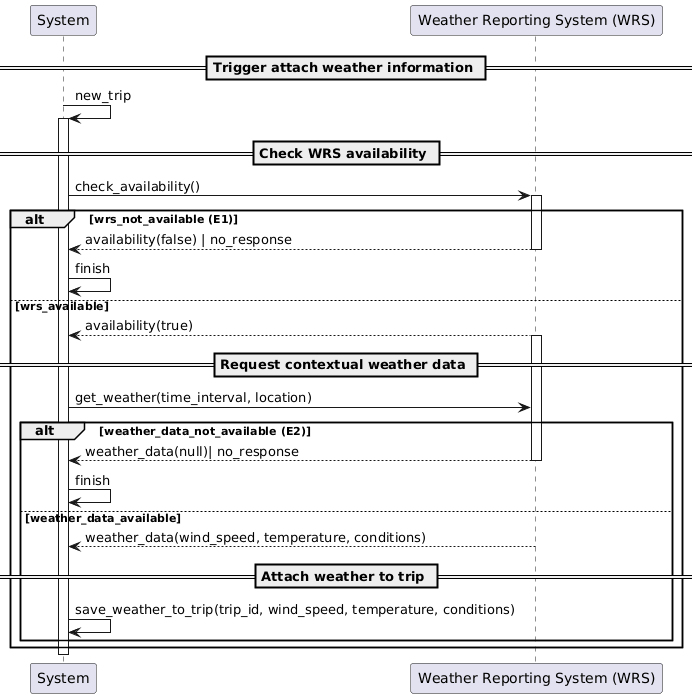
\includegraphics[width=\textwidth]{Images/Diagrams/Sequence/attach_weather.png}
\caption{\label{fig:squencediagram}Sequence diagram for attach weather information.}
\end{figure}

\pagebreak

\item \textbf{Review a trip}

\begin{figure}[H]
\centering
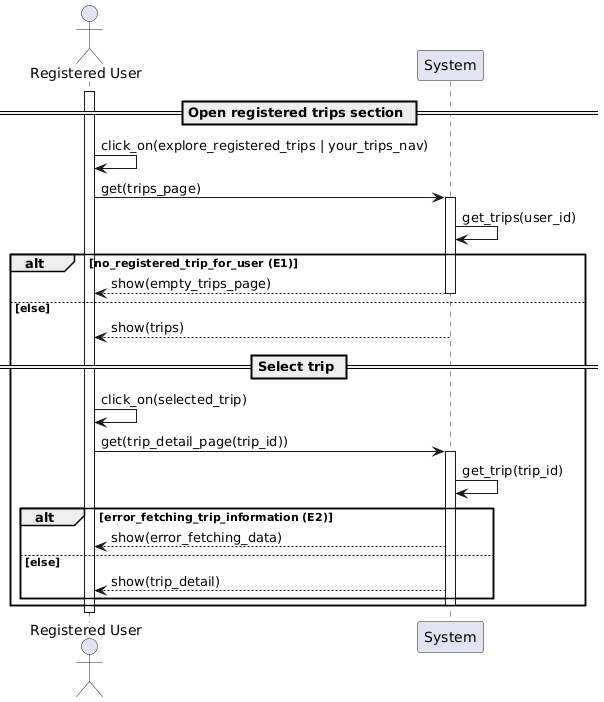
\includegraphics[width=\textwidth]{Images/Diagrams/Sequence/review_trip.png}
\caption{\label{fig:squencediagram}Sequence diagram for review trip.}
\end{figure}

\pagebreak

\item \textbf{Enable Automated Mode}

\begin{figure}[H]
\centering
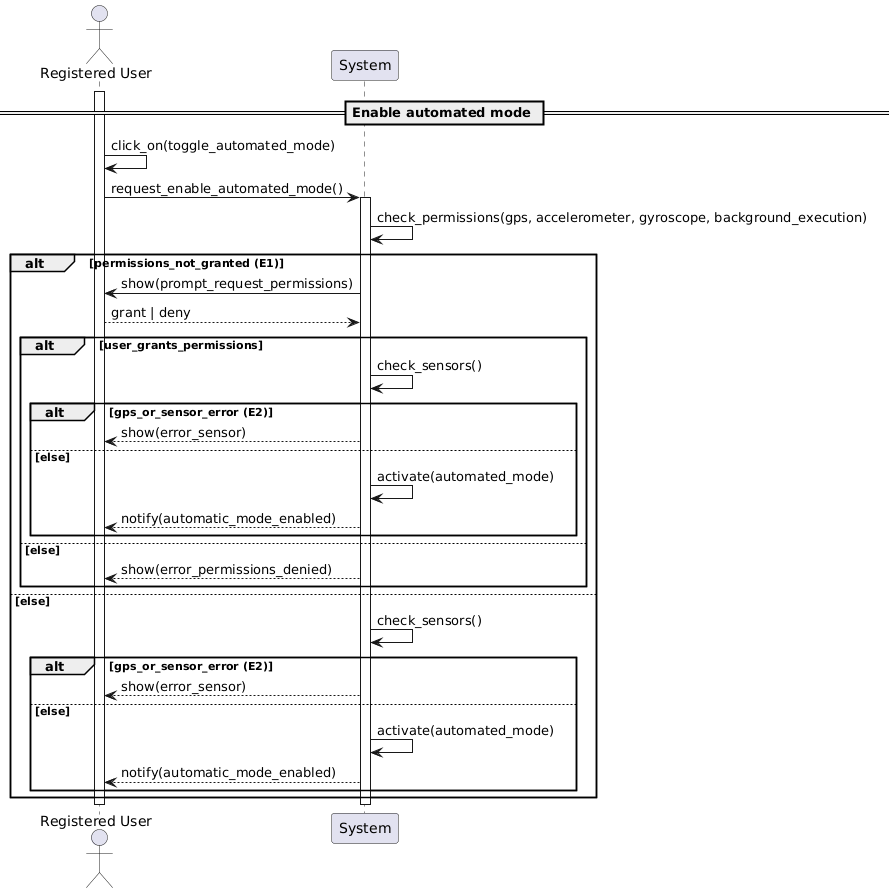
\includegraphics[width=\textwidth]{Images/Diagrams/Sequence/enable_auto_mode.png}
\caption{\label{fig:squencediagram}Sequence diagram for enable automated mode.}
\end{figure}

\pagebreak

\item \textbf{Disable Automated Mode}

\begin{figure}[H]
\centering
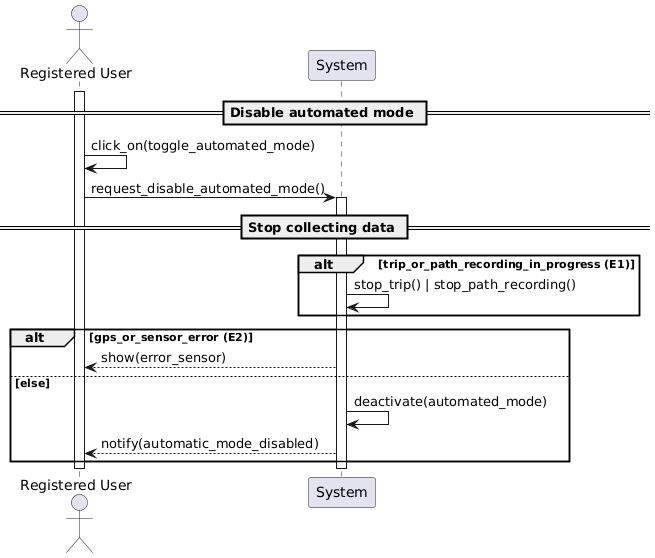
\includegraphics[width=\textwidth]{Images/Diagrams/Sequence/disable_auto_mode.png}
\caption{\label{fig:squencediagram}Sequence diagram for disable automated mode.}
\end{figure}

\pagebreak

\item \textbf{Record a Path in Manual Mode}

\begin{figure}[H]
\centering
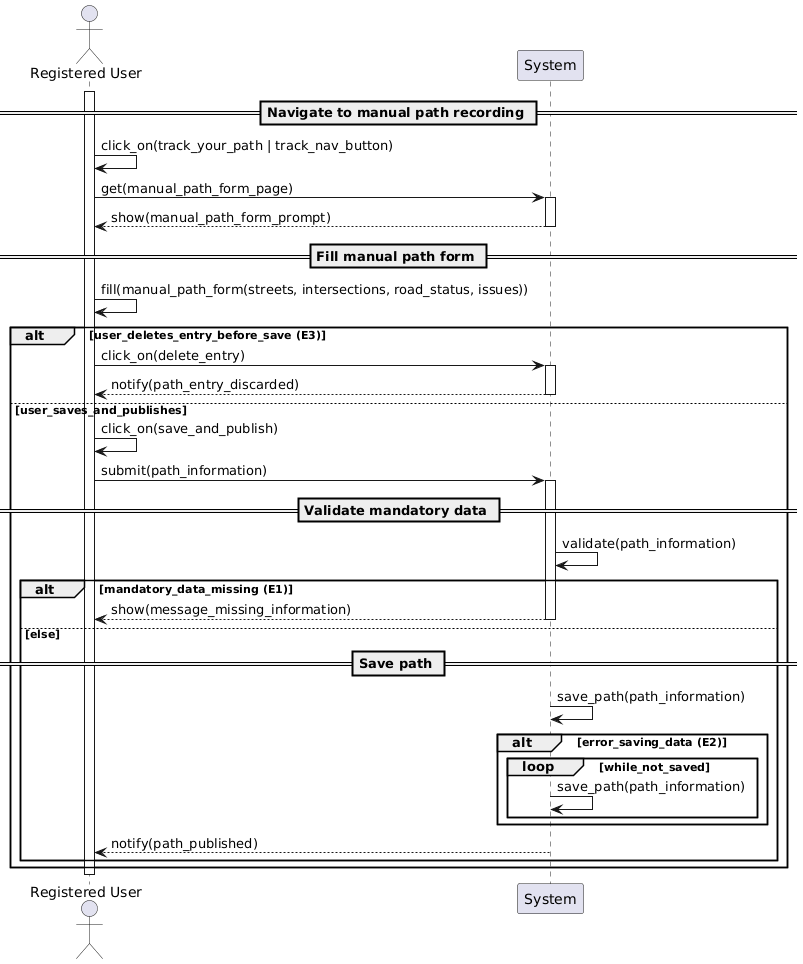
\includegraphics[width=\textwidth]{Images/Diagrams/Sequence/publish_path_manual_mode.png}
\caption{\label{fig:squencediagram}Sequence diagram for record a path in manual mode.}
\end{figure}

\pagebreak

\item \textbf{Record a Path in Automated Mode}

\begin{figure}[H]
\centering
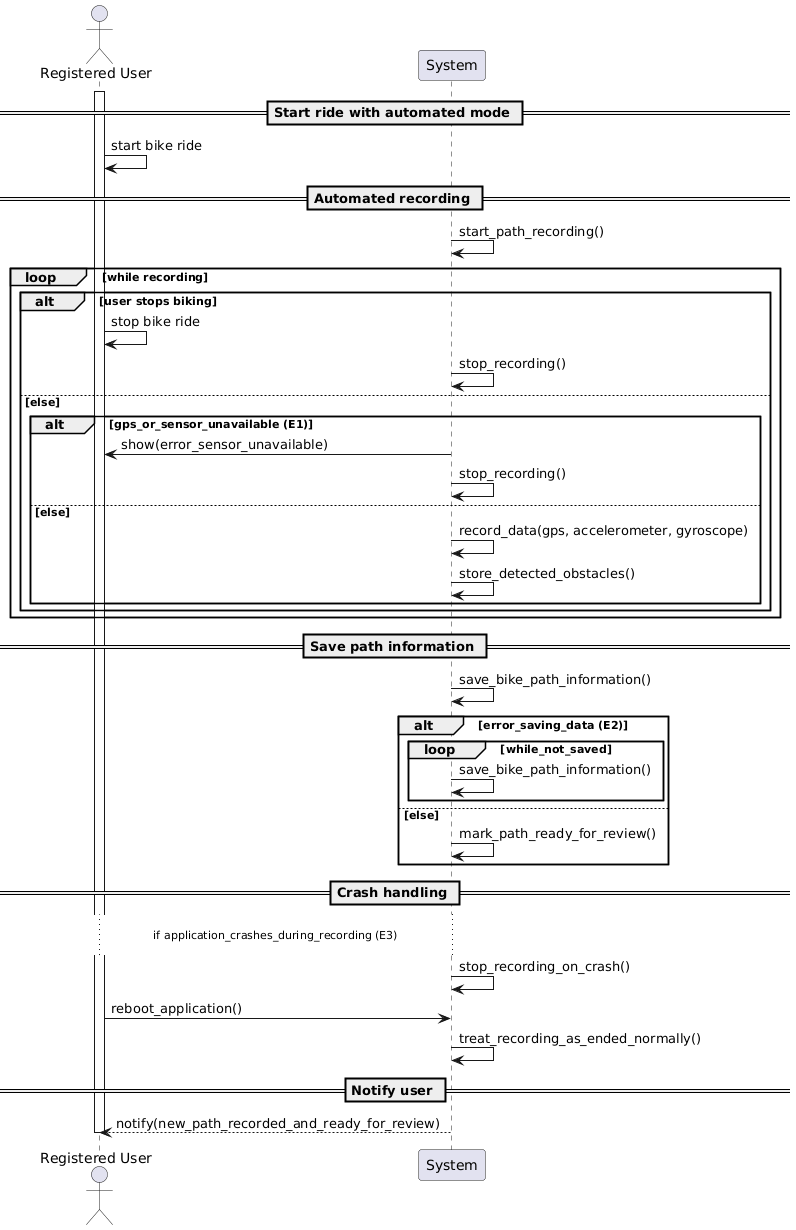
\includegraphics[scale=0.5]{Images/Diagrams/Sequence/record_path_automated.png}
\caption{\label{fig:squencediagram}Sequence diagram for record a path in automated mode.}
\end{figure}

\pagebreak

\item \textbf{Publish a pre-recorded automated mode path}

\begin{figure}[H]
\centering
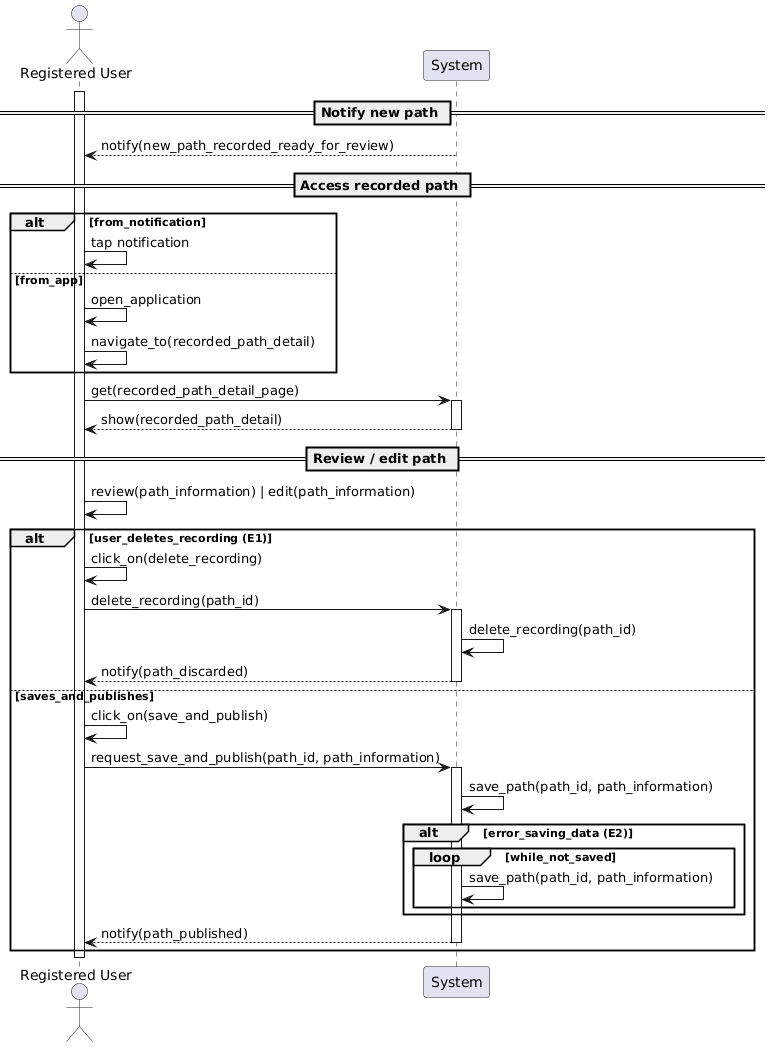
\includegraphics[width=\textwidth]{Images/Diagrams/Sequence/publish_path_auto_mode.png}
\caption{\label{fig:squencediagram}Sequence diagram for publish a pre-recorded automated mode path.}
\end{figure}

\pagebreak

\item \textbf{Logout}

\begin{figure}[H]
\centering
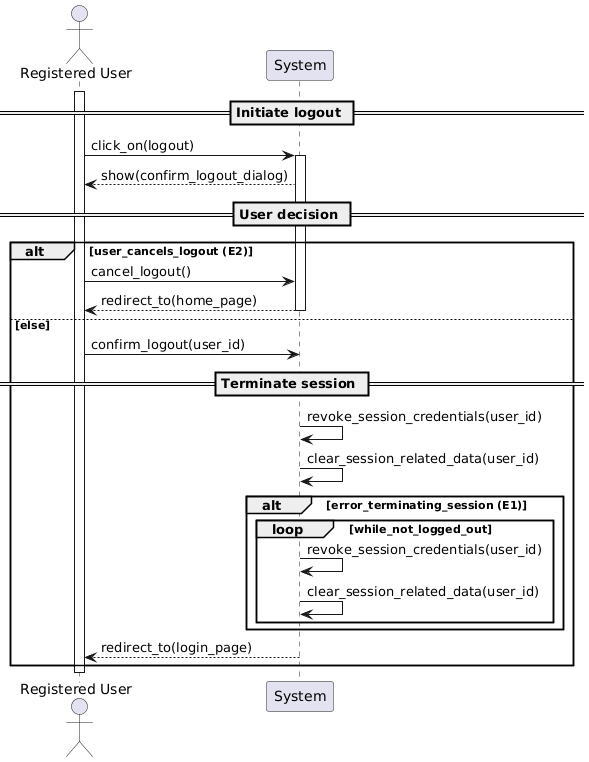
\includegraphics[width=\textwidth]{Images/Diagrams/Sequence/logout.png}
\caption{\label{fig:squencediagram}Sequence diagram for logout.}
\end{figure}

\pagebreak



\end{enumerate}

\subsection{Performance Requirements}
The system must be designed to handle a large number of concurrently connected and registered users, making scalability one of its primary functional requirements. As the platform is expected to serve many users at a time from many devices, it must be able to expand seamlessly while keeping performance degradation to a minimum. In other words, despite the number of users that use the different functionalities of the System, this still has to be reliable and stable.

Availability is equally essential: due to one of the functionality of the system being a "searching for paths" one, the uptime must be maximized and deliver information rapidly and efficiently. Key features such as search, tailored paths, and publishing processes must guarantee low response times and avoid introducing operational bottlenecks in such events, especially at peak of requests and high number of paths submitted. In addition, the system must support the upload and management of substantial volumes of metadata of the user paths, without compromising responsiveness or stability in the publish processing, but even when the automated mode is activated and user (taken account it is registered) is currently riding. 

Furthermore, any possible estimation of active users on the platform is hard to get, as there are many competitors that deals only with specific functionalities of BBP. To give an example, if we consider Strava's platform that deals with trip metrics, there are estimation of around 40-50 millions monthly users ~\cite{StravaYearInSport2025}. So, as a simple comparison (that takes account the part that gather trip information), BBP is supposed to cope with a number of concurrent users around 30.000, assuming an hypothetical average of two hours of usage per access. However, it is also reasonable to state that this estimation does not take account of the variance of such values, as there might be periods of the year with much greater accesses, and others with smaller ones. As a result, usage cannot be considered exclusively stable but, instead, a value that might oscillate. 

\subsection{Design Constraints}
\subsubsection{Standards compliance}
{Conformity Standards}
\begin{enumerate}
\item GDPR: The system should manage user data, location tracking and data path in the European Union, thus it is compliant with the General Data Protection Regulation according to the European guidelines.
\item Local privacy laws: The System should manage user data, location tracking and data path, thus it is compliant with the local laws in countries outside the European Union.
\item ISO/IEC 27001 ~\cite{ISOIEC27001}: The system must adopt structured and comprehensive information security management, in order to protect sensitive information and be adaptable to new risks.
\item ISO/IEC 25010 ~\cite{ISOIEC25010}: The system must be developed as to follow proper quality standards for reliability, performance, maintainability, and security.
\end{enumerate}
{Development Standards}
\begin{enumerate}
\item ISO/IEC 12207 ~\cite{ISOIECIEEE12207}: The system must apply the best practices in all the main processes that bring to its realization, in full compliant with the software life-cycle management standards.
\end{enumerate}
\subsubsection{Hardware Limitation}
\begin{enumerate}
\item In order for the application to work properly, the devices must be able to allocate enough resources to the background processes. In other words, a good CPU and enough RAM are needed. Minimum requirements like a quad-core processor is needed as a reliable resource for background activities. Furthermore, 4 GB of Ram is needed but for multi-tasking processes more of that is suggested. Long paths, especially for those taking hours, might affect the battery life-cycle of the device, especially if the automated mode is activated, as the usage of sensors is highly expensive in terms of battery consumption. As a result, battery devices shall be recent or have high volume capacity in order to avoid any early shutdown, leading the device to shut down the ongoing path data collection. 
\item Sensors, especially for the automated mode, are strictly necessary such as, gyroscopes, GPS sensors or even GNSS equivalent and accelerometer. Drivers shall be updated in order to use properly those sensors. 
\item In terms of software requirements, devices must provide the rights to the application to use most of the features in background in order to collect data of the path, as mentioned before. As a result, only latest versions of OS should be considered. However, as minimal requirements, in terms of Android Environment, require Android 10, that supports foreground-services and location authorizations in background, as might be limited in previous versions. For similar reasons, even in Apple environment, a minimum iOS version must be considered, by considering iOS 13, as it provides improved location tracking in background.
\item In terms of data collection, the System collects all the user data and the related path. As a result, the System should be able to  provide consistency and reliability in terms of paths scores and analysis. This is because, a good DBMS, especially an hybrid one, provide a good mixture of qualities of relational and non-relational models, as the System has to deal with different types of data, and concurrently also provide flexibility and high responsiveness.
\end{enumerate}

\subsubsection{Any other constraint}

In terms of connectivity, devices should rely on wireless infrastructures in order to send and receive data in case of collection of data, search and publication of paths. So, this is mostly an external party that affects, however, the user experience of the application as an overall. 

\subsection{Software System Attribute}
The BBP system must satisfy several key software attributes to ensure reliability, usability, and overall performance.     
\subsubsection{Scalability}
The most critical element is scalability as the system must efficiently handle a large number of registered and anonymous users simultaneously. In fact, the most costly effort is to decrease as much as possible the performance degradation even under peak usage. The system should manage new user registration and any surge of signs up. So the systems as a overall is supposed to be well efficiently structured.
\subsubsection{Availability}
As a result of Scalability, Availability is even crucial. The Search mode for bike paths requires to handle many sets of data already stored and organized in schema by the DBMS. As a result, the system must remain responsive and accessible at all times, delivering information quickly even at the highest peak of usage. Not to mention that the system must also provide robustness and fault tolerance. So, the system has to ready and able to manage many accesses at a time. If we consider periods of time when weather is especially suitable for riding, we expect to have peak of usage in the late morning (9:00 - 12:00) and late afternoon (17:00 - 20:00) between April and September. BBP is expected to be available, accessible and ready.
\subsubsection{Reliability}
The system should rely on a robust backup and recovery infrastructure capable of preserving data integrity at all times, even in the presence of unexpected faults. All critical elements must exhibit high reliability, so the architecture should incorporate redundant and parallelized components, ensuring that the failure of a single node, service, or storage unit does not compromise the availability of the platform.
\subsubsection{Security and privacy}
 Security is particularly important in terms of paths that are not directly related to the users, once published. Sensitive information must be stored and transmitted securely respecting user anonymity. In fact, data must be well stored and restricted accessed, preventing backdoor access and similar events. Furthermore, as GPS location is essential in the automated mode, user privacy is one of the most important aspect to mention. Given the sensitive nature of the information handled such that, every piece of user-related data must be protected with modern, robust cryptographic techniques. Only algorithms that are still considered secure by current standards should be used, such as hashing functions with adequate resistance like SHA-256, and encryption schemes such as AES-256 to safeguard stored content. 
 \subsubsection{Maintainability}
 In order to update the system in future and take account of additional new features, maintainability is then crucial, as well as an structured modular architecture. Furthermore, even a documentation for the related code should be clear, complete and easy to those in charge to maintain the system in future. Additionally, the project should adopt standard development practices such as version control workflows ( such as Git flow), automated testing, continuous integration/continuous delivery (CI/CD), and coding style guidelines. These practices reduce technical debt, improve code quality, and make sure that updates can be introduced safely and efficiently.
 \subsubsection{Portability}
 The system should be designed to be accessible and installed on operating systems such as iOS and Android. As a result, all the designed features should be all available, independently on the OS been used. Finally, the installation and update process should follow each platform’s best practices, ensuring seamless deployment via official app stores, secure updates, and minimal friction for the user.

